\section{METODOLOGIA}
Neste projeto de pesquisa foi empregado diversos modelos de aprendizagem profunda, tais como \ac{FCN}, \ac{U-Net}, \ac{SegNet} e \ac{MobileNetV2}, para segmentar feridas malignas em imagens médicas. Utilizaremos um grande conjunto de dados que reuniu uma junção de vários dataset de feridas. As imagens, que apresentam diversas formas e variações, serão pré-processadas antes do treinamento. Avaliaremos quantitativamente a performance dos modelos com base na área da ferida, precisão e eficiência do modelo na segmentação das imagens. A Figura~\ref{fig:diagrama} demonstra o fluxograma da metodologia aplicada.

\begin{figure}[htbp]
    \centering
    \caption{Diagrama da Metodologia}
    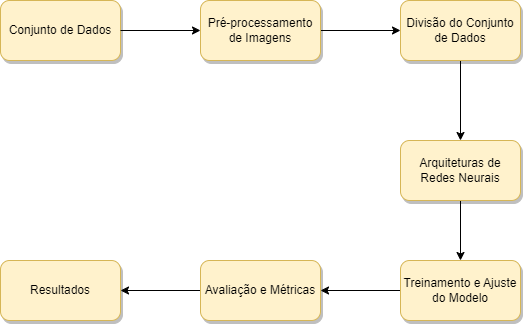
\includegraphics[width=0.8\textwidth]{img/Diagrama.png}
    \label{fig:diagrama}
    \par\medskip\textbf{Fonte:} Autor
\end{figure}

\subsection{Conjunto de Dados}
    O conjunto de dados deste estudo compreende imagens de feridas malignas coletadas de diversas fontes, incluindo repositórios públicos no GitHub e sites especializados em imagens médicas. Selecionamos mais de 4.800 imagens para treinar, validar e testar os modelos de aprendizado profundo, considerando a diversidade de tipos de feridas malignas e a qualidade das imagens. A utilização de um conjunto de dados amplo e diversificado contribuirá para aprimorar os resultados deste estudo e desenvolver modelos de aprendizado profundo mais eficazes na segmentação de feridas malignas.
    
\subsection{Criação do Conjunto de Dados}
    
    \begin{itemize}
        \item Tipo de imagens: As imagens médicas incluídas neste conjunto abrangem diversos tipos, tais Feridas de úlceras em pé diabéticos, lesões com cortes profundas e feridas crônicas em diversas partes do corpo. Suas características, como resolução, dimensões e formato de arquivo, são especificadas para proporcionar uma compreensão detalhada. Detalhamos o processo de aquisição, incluindo informações sobre o equipamento utilizado, configurações e protocolos adotados para a captura dessas imagens médicas.
    
        \item Pré-processamento e Anotação: Descrevemos as técnicas de pré-processamento aplicadas, como normalização e aumento de dados, ressaltando a importância dessas etapas na preparação das imagens para análise. O processo de anotação é abordado, incluindo responsáveis e critérios utilizados. Foi abordado nos dados sobre a diversidade do conjunto, considerando variabilidade em condições médicas, faixas etárias, gêneros e outros fatores relevantes, garantindo representatividade.
    
        \item Volume de Dados: Informamos a quantidade total de imagens e casos incluídos no dataset, proporcionando uma visão abrangente de sua robustez e amplitude. Consideramos mais de 4.800 imagens no dataset de diferentes fontes públicas e de diferentes condições clínicas para atender a heterogeneidade dos dados.
    
        \item Questões Éticas e de Privacidade: Abordamos as questões éticas, incluindo o consentimento informado, os processos de anonimização de dados e a conformidade com regulamentos de privacidade e proteção de dados.

        \item Qualidade e Confiabilidade dos Dados: Sobre a qualidade das imagens, considerando resolução e clareza, e a confiabilidade das anotações. Destacamos qualquer validação realizada por especialistas médicos para assegurar a precisão.

        \item Disponibilidade e Acesso: Fornecemos informações sobre a disponibilidade pública do dataset, incluindo detalhes sobre como acessá-lo, bem como eventuais restrições ou requisitos associados.

        \item Potenciais Aplicações e Limitações: Descrevemos possíveis aplicações do conjunto de dados em modelos de visão computacional, destacando suas potencialidades. Além disso, discutimos abertamente quaisquer limitações conhecidas ou possíveis viéses que devem ser considerados durante o uso do dataset.

        
    \end{itemize}

\subsection{Pré-processamento de Imagens}

    As imagens foram inicialmente redimensionadas para uma resolução de 256x256 pixels para normalizar o tamanho da imagem e facilita o processamento de acordo com vários modelos. Os valores de píxel foram então normalizados para um intervalo de 0 a 1 para garantir uma escala de intensidade consistente em todas as imagens.

    Além disso, técnicos de aumento de dados, como rotação, inversão horizontal e dimensionamento É usado para aumentar a diversidade de conjuntos de dados e evitar overfitting. Essas técnicos permitem que os modelos aprendem a reconhecer as características das lesões malignos em diferentes locais e escalas.

    Vale ressaltar que nenhum filtro de suavização foi aplicado nas imagens para preservar as características originais das feridas. Isto é crucial para garantir que os modelos aprendem a reconhecer as especificidades das lesões malignos e não sejam afetados por artefatos de imagem. Estas são fases críticas no treinamento de modelos de Machine Learning para identificar lesões malignos. Eles permitem que os modelos aprendem a reconhecer as especificidades das lesões malignos de forma mais flexível e precisa, resultando em segmentações mais precisos e confiáveis.

\subsection{Divisão do Conjunto de Dados}
    A divisão do conjunto de dados foi realizada de forma estratificada, garantindo uma distribuição uniforme das classes de feridas malignas em cada subconjunto. Essa metodologia é crucial para manter a representatividade e o equilíbrio do conjunto de dados, minimizando possíveis viéses e reforçando a confiabilidade dos resultados. O conjunto foi dividido em dois grupos principais: treinamento e teste. O grupo de treinamento desempenhou um papel vital no processo de aprendizagem dos modelos de aprendizado profundo, enquanto o grupo de teste foi empregado para avaliar a eficácia dos modelos em dados novos e não vistos anteriormente. A divisão foi realizada aleatoriamente, mas com o cuidado de manter as proporções de cada classe de feridas malignas em cada segmento. Esse cuidado assegura que tanto o treinamento quanto a avaliação dos modelos ocorram em um ambiente de dados bem balanceado e representativo, crucial para a obtenção de resultados confiáveis e precisos.

\subsection{Arquiteturas de Redes Neurais}
    Para realizar a segmentação das feridas malignas cutâneas, foram exploradas quatro arquiteturas de redes neurais convolucionais:

    \subsubsection{FCN}
    
        A arquitetura \ac{FCN}, representada abaixo na figura \ref{fig:arquiteturaFCN},  é conhecida por sua capacidade de realizar a segmentação semântica em imagens. Ela consiste em uma rede neural convolucional totalmente composta por camadas convolucionais, sem camadas totalmente conectadas. 

        \clearpage
        
        \begin{figure}[htbp]
            \centering
            \caption{Representação Esquemática da Arquitetura \ac{FCN}.}
            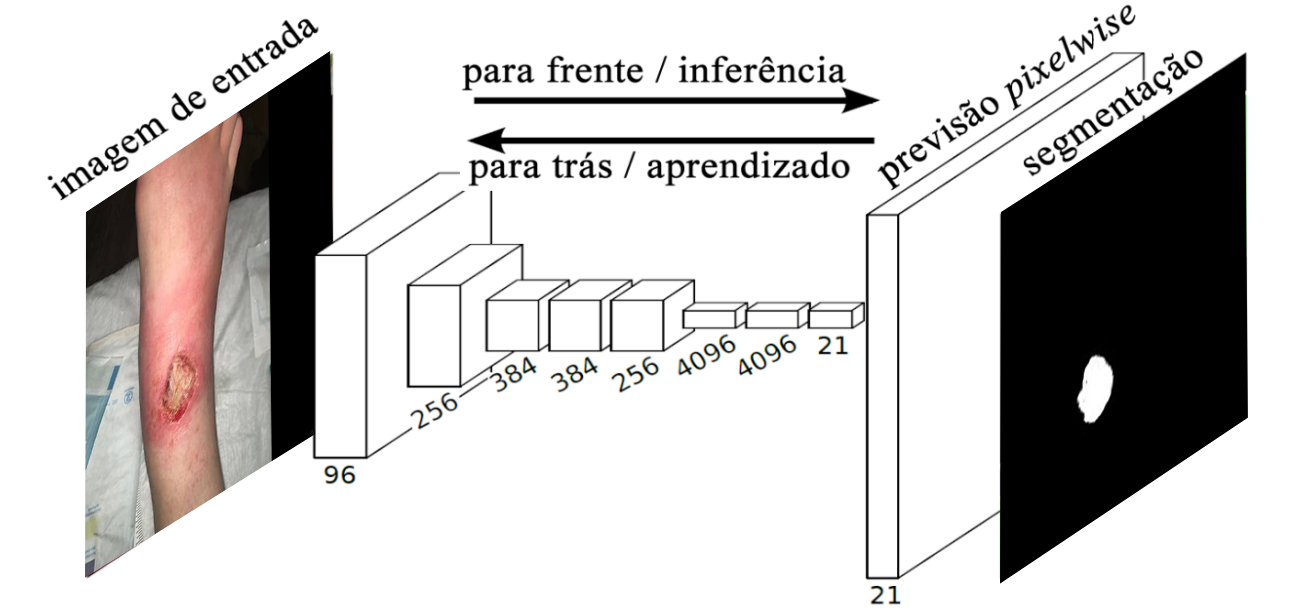
\includegraphics[width=0.8\textwidth]{img/arquitetura_FCN.png}
            \label{fig:arquiteturaFCN}
            \par\medskip\textbf{Fonte:} adaptada de (\cite{long2015fully})
        \end{figure}
        
        A Figura \ref{fig:arquiteturaFCN} acima, apresenta a arquitetura de uma rede \ac{FCN} utilizada para tarefa de segmentação semântica (semantic segmentation), isto é, classificar cada pixel da imagem de entrada de acordo com a classe que ele pertence, sendo: cama, pé ou ferida (background). Conforme a arquitetura apresentada na Figura, existem várias camadas de convolução que produzirão mapas de características de diferentes profundidades. No final da rede, encontra-se a previsão pixelwise (pixelwise prediction) que também é um tipo de camada de convolução e que irá fazer uma predição pixel-a-pixel, isto é, atribuindo cada pixel a uma respectiva classe. Esta representação ilustra de forma esquemática a arquitetura \ac{FCN}, mostrando as camadas convolucionais e suas dimensões. Essa arquitetura é capaz de extrair as características mais importantes das imagens de feridas malignas, permitindo que a rede aprenda a segmentar essas feridas com precisão. 



    
    \subsubsection{U-Net}

        A arquitetura \ac{U-Net}, ilustrada na figura \ref{fig:arquiteturaUNet} abaixo,  é amplamente utilizada para tarefas de segmentação em imagens biomédicas. Ela possui uma estrutura em forma de U, com um encoder para capturar informações contextuais e um decoder para reconstruir a máscara de segmentação. A \ac{U-Net} é conhecida por sua capacidade de segmentação precisa e é aplicada com sucesso em diversos problemas de segmentação, incluindo a segmentação de feridas medicas.

        \clearpage

        \begin{figure}[htbp]
            \centering
             \caption{Representação Esquemática da Arquitetura \ac{U-Net}. }
            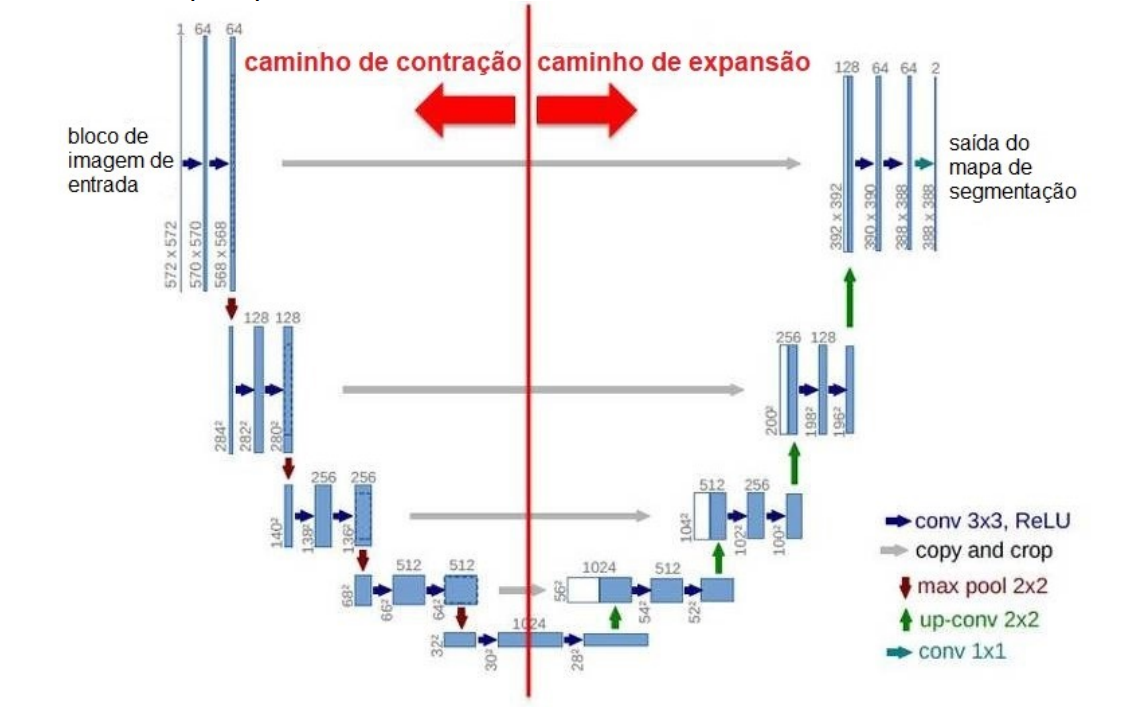
\includegraphics[width=0.8\textwidth]{img/arquitetura_U-Net.png}
            \label{fig:arquiteturaUNet}
            \par\medskip\textbf{Fonte:} adaptada de (\cite{ronneberger2015u})
        \end{figure}

            A Figura \ref{fig:arquiteturaUNet} acima, ilustra a arquitetura da rede \ac{U-Net}, em que cada caixinha azul presente na imagem corresponde a um mapa de característica multicanal (multichannel feature map). O número de cada canal está descrito no valor acima de cada caixa. No canto inferior esquerdo é dada a dimensão x-y da imagem. As caixas brancas representam a cópia dos mapas de características (feature maps) e cada flecha com sua respectiva cor representa uma operação diferente. Na parte direita da rede as flechas verdes referem-se ao caminho de expansão onde é utilizado a operação de up-convolution, também chamada de de-convolution6 ou transposed convolution. A figura ilustra essa arquitetura de forma esquemática, mostrando as camadas convolucionais, as camadas de pooling máximo e up-sampling, e as conexões laterais entre as camadas do caminho de contração e do caminho de expansão.


    
    \subsubsection{SegNet}

        O modelo \ac{SegNet}, representado na figura \ref{fig:arquiteturaSegNet} abaixo,  é baseado em uma arquitetura de codificador-decodificador. Cada codificador aplica convolução, normalização de lote e uma não linearidade, e depois aplica um pool máximo no resultado, enquanto armazena o índice do valor extraído de cada janela. Os decodificadores são semelhantes aos codificadores, a diferença é que eles não têm uma não linearidade e aumentam a amostra de entrada, usando índices armazenados a partir do estágio de codificação.

        \clearpage

        \begin{figure}[htbp]
            \centering
            \caption{Representação Esquemática da Arquitetura \ac{SegNet}.}
            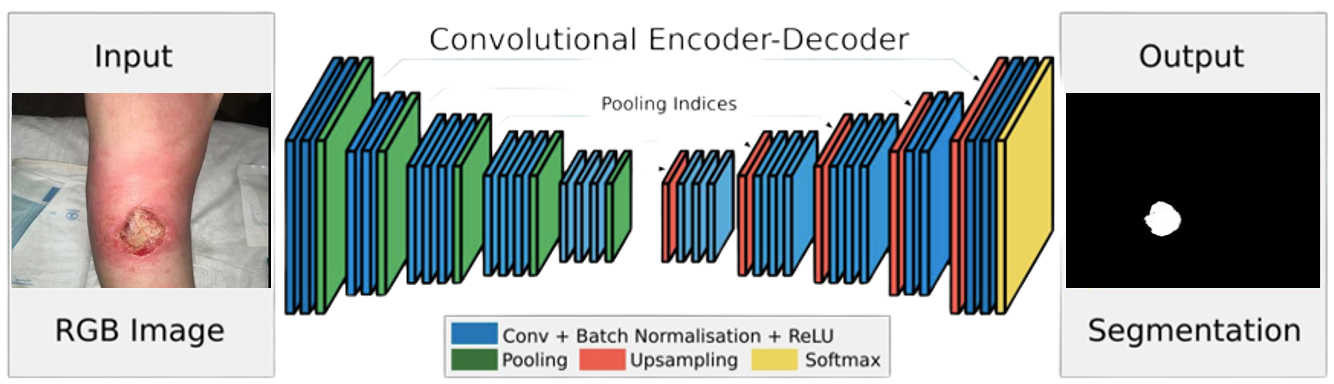
\includegraphics[width=0.9\textwidth]{img/arquitetura_Seg-Net.png}
            \label{fig:arquiteturaSegNet}
            \par\medskip\textbf{Fonte:} adaptada de (\cite{badrinarayanan2017deep})
        \end{figure}

            A Figura \ref{fig:arquiteturaSegNet} acima, ilustra essa arquitetura de forma esquemática, mostrando as camadas de codificação e decodificação, bem como as conexões entre elas. Cada caixa na figura representa uma camada de convolução, normalização de lote e não linearidade, enquanto as setas representam as conexões entre as camadas. As camadas de pooling máximo são representadas pelas caixas de cor verde. Além disso, a figura também mostra a saída da rede, que é uma imagem segmentada com as áreas de feridas malignas destacadas em branco. Essa saída é gerada pela última camada de decodificação da rede.
            Em resumo, a Figura ilustra de forma esquemática a arquitetura \ac{SegNet}, mostrando as camadas de codificação e decodificação, bem como as conexões entre elas. Essa arquitetura é capaz de segmentar com precisão as feridas malignas em imagens médicas, como mostrado nos resultados do estudo.

    \clearpage
    
    \subsubsection{MobileNetV2}

        O \ac{MobileNetV2}, representada na figura \ref{fig:arquiteturaMobileNetV2} abaixo, é uma arquitetura de rede neural convolucional projetada para tarefas de classificação e segmentação em dispositivos com recursos computacionais limitados. Essa arquitetura utiliza camadas convolucionais separáveis em profundidade para obter um bom equilíbrio entre a precisão do modelo e a eficiência computacional.
    
            \begin{figure}[htbp]
                \centering
                \caption{Representação Esquemática da Arquitetura \ac{MobileNetV2}.}
                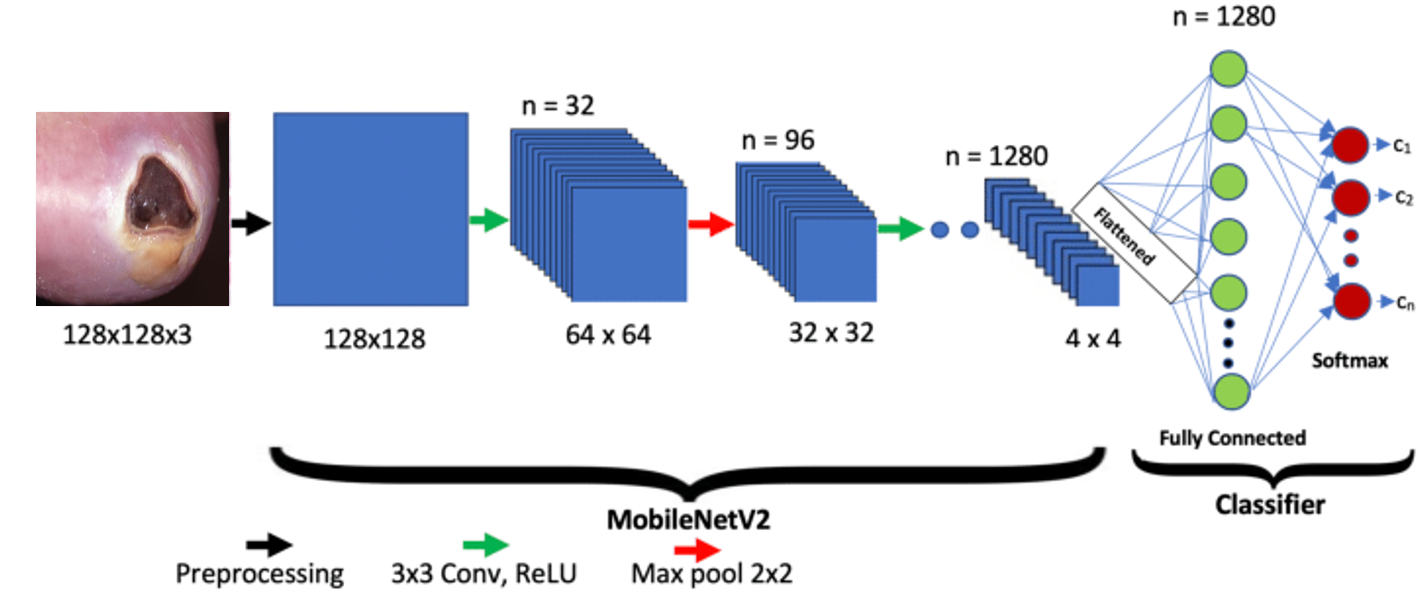
\includegraphics[width=0.8\textwidth]{img/arquitetura_MobileNetV2.png}
                \label{fig:arquiteturaMobileNetV2}
                \par\medskip\textbf{Fonte:} adaptada de (\cite{akay2021deep})
            \end{figure}   
    
        A figura \ref{fig: arquiteturaMobileNetV2} mostra esquematicamente esta arquitetura. Revela a camada de convolução e seu tamanho. A imagem de entrada é uma imagem de ferida com dimensões 128x128x3, que é processada pela primeira camada convolucional com dimensões 128x128 e um número de filtros (ou canais) igual a 32. Em seguida a imagem é processada por uma segunda camada convolucional com dimensões 64x64 e uma número de filtros igual a 32. Em seguida, a imagem é processada por diversas camadas convolucionais com dimensões 32x32 e 96 filtros, que são responsáveis por extrair características mais complexos da imagem Estas camadas são seguidas por uma camada convolucional de dimensões 4x4 e um número de filtros igual a 1280, responsáveis por extrair as características mais importantes da imagem Por fim, a saída da última camada convolucional é processada por uma rede totalmente conectada com número de neurônios igual a 1280, que é responsável por gerar a saída final da rede.

\subsection{Treinamento e Ajuste do Modelo}

    Durante o treinamento, uma série de imagens de feridas malignas é usada para ensinar o modelo a segmentar com precisão essas feridas. Ao fazer isso Dividimos o conjunto de imagens em um conjunto de treinamento e um conjunto de teste. e usar técnicos de aumento de dados para aumentar a diversidade do conjunto de treinamento.

    Adicionalmente, aplicamos técnicos de poda ao modelo discutido com o objetivo de reduzir o número de parâmetros e melhorar a eficiência computacional do modelo. A técnica de poda consiste em retirar os pesos mais importantes do modelo e reter apenas os pesos mais importantes. Isso aumenta a memória e o desempenho de processamento do modelo sem degradar a precisão da segmentação.

    O processo de otimização usa o conjunto de dados para otimizar os hiperparâmetros do modelo e evitar overfitting. Ajuste hiperparâmetros como taxa de aprendizado, tamanho do lote e número de eras de treinamento para obter a maior precisão de segmentação possível.

\subsection{Avaliação e Métricas}
    Para avaliar a eficácia dos modelos de segmentação de lesões malignas em imagens médicas, aplicou-se um conjunto de métricas essenciais. Utilizou-se a métrica de Loss para quantificar a discrepância entre as segmentações previstas pelos modelos e as reais, com valores menores indicando maior precisão na segmentação. A métrica Dice, que avalia a sobreposição entre as previsões do modelo e a verdade padrão, é outra ferramenta crucial, onde resultados mais próximos de 1 representam uma sobreposição ideal. Precisão, que mede a exatidão do modelo na identificação correta das lesões malignas, esse métrica avalia a proporção de verdadeiros positivos frente às predições positivas. Essas métricas conjuntas proporcionam uma análise detalhada do desempenho, orientando ajustes e melhorias. Valores ideais são definidos conforme as demandas clínicas, assegurando a confiabilidade dos processos de segmentação. A extensão das lesões foi quantificada, e testes estatísticos t foram utilizados para discernir diferenças significativas entre os modelos. Essa metodologia abrangente garante uma avaliação precisa dos modelos de segmentação, crucial para a prática médica.

\subsection{Considerações Éticas}

    Dado as diretrizes das imagens médicas de pacientes, atendemos rigorosamente às considerações éticas. Anonimizaremos todas as imagens, removendo dados identificáveis para assegurar a privacidade dos pacientes. Este projeto caminhou para atender as diretrizes da Declaração de Helsinque para pesquisas envolvendo seres humanos. Essa declaração é um conjunto de princípios éticos que orientam a pesquisa médica envolvendo seres humanos.
    
    A implementação desta metodologia permitirá avaliar a eficácia de vários modelos de aprendizagem profunda na segmentação de feridas malignas em imagens médicas. Compararemos os modelos usando uma variedade de métricas para fornecer insights valiosos para o desenvolvimento de futuros sistemas de diagnóstico assistido por computador na área de oncologia cutânea.

